\documentclass[10pt,a4paper]{article}
\usepackage[a4paper]{geometry}
\usepackage[english]{babel}
\usepackage{amsmath}
\usepackage{amsfonts}
\usepackage{amssymb}
\usepackage{makeidx}
\usepackage{graphicx}
\usepackage{caption}
\usepackage{subcaption}
\usepackage{color}
\usepackage{import}

\usepackage{epstopdf}

\title{Les exemples du cours}
\author{Matthew OZON} %, \href{mailto:matthew.ozon@cpe.fr}{matthew.ozon@cpe.fr}
\date{\today}

%begining of the document
\begin{document}
\maketitle

\section{Histoire}

\section{Les op\'{e}rateurs : resum\'{e}es}

\subsection{Translation et transpos\'{e}e d'ensemble}
\paragraph{Translation} L'op\'{e}ration la plus basique entre un ensemble $X$ et un vecteur $B$ que l'on note $X_b$: 
\begin{displaymath}
	X_b = \{x+b|x\in X\}
\end{displaymath}

\paragraph{Transpos\'{e}}
Operation qui transforme tout point en son ``opos\'{e}'', relativement \'{a} une origine. Pour un ensemble $X$, on note $X^t$ son transpos\'{e} qui est d\'{e}fini par : 
\begin{displaymath}
	X^t = \{-x | x\in X\}
\end{displaymath}

\subsection{addition et soustraction de Minkowski : les op\'{e}rateurs de dilatation et d'\'{e}rosion}

L'addition et la soustraction de Minkowski sont d\'{e}finit comme suit pour deux ensembles $X$ et $B$ :

\begin{align*}	
	X\oplus B &= \{x+b | x\in X, b\in B\} = \cup\{X_b | b\in B\} 	\\
	X\ominus B &= \{x | B_{-x}\subseteq X\} = \cap\{X_b | b\in B\}
\end{align*}

et les op\'{e}rateurs de dilatation et d'\'{e}rosion sont :
\begin{align*}	
	D_{B}\left(X\right) &= X\oplus B^t	\\
	E_{B}\left(X\right) &= X\ominus B^t
\end{align*}


Quelques propri\'{e}t\'{e}s int\^{e}ressantes de la dilatation et de l'\'{e}rosion : 
\begin{itemize}
	\item extensivit\'{e} : $E_B\left(X\right) \subseteq X \subseteq D_B\left(X\right)$ 
	\item croissance : $X\subset Y \Rightarrow E_B\left(X\right) \subset E_B\left(Y\right) \text{ et } D_B\left(X\right) \subset D_B\left(Y\right)$
	\item distributivit\'{e} : $E_B\left(X\cap Y\right) = E_B\left(X\right) \cap E_B\left(Y\right)$ et $D_B\left(X\cup Y\right) = D_B\left(X\right) \cup D_B\left(Y\right)$
	\item connexit\'{e} : non pr\'{e}serv\'{e}e par les deux op\'{e}rateurs.
	\item composition : $D_{B_2}\left(D_{B1}\left(X\right)\right) = D_{D_{B_{2}^{t}\left(B_1\right)}}\left(X\right)$ et  $E_{B_2}\left(E_{B1}\left(X\right)\right) = E_{D_{B_{2}^{t}\left(B_1\right)}}\left(X\right)$ 
	\item dualit\'{e} : $ E_B\left(X\right) = \overline{ D_B\left(\overline{X}\right)}$
\end{itemize}

\begin{figure}[h]
	\centering
\scalebox{0.45}{% Title: glps_renderer figure
% Creator: GL2PS 1.3.8, (C) 1999-2012 C. Geuzaine
% For: Octave
% CreationDate: Tue Nov 18 11:12:08 2014
\setlength{\unitlength}{1pt}
\begin{picture}(0,0)
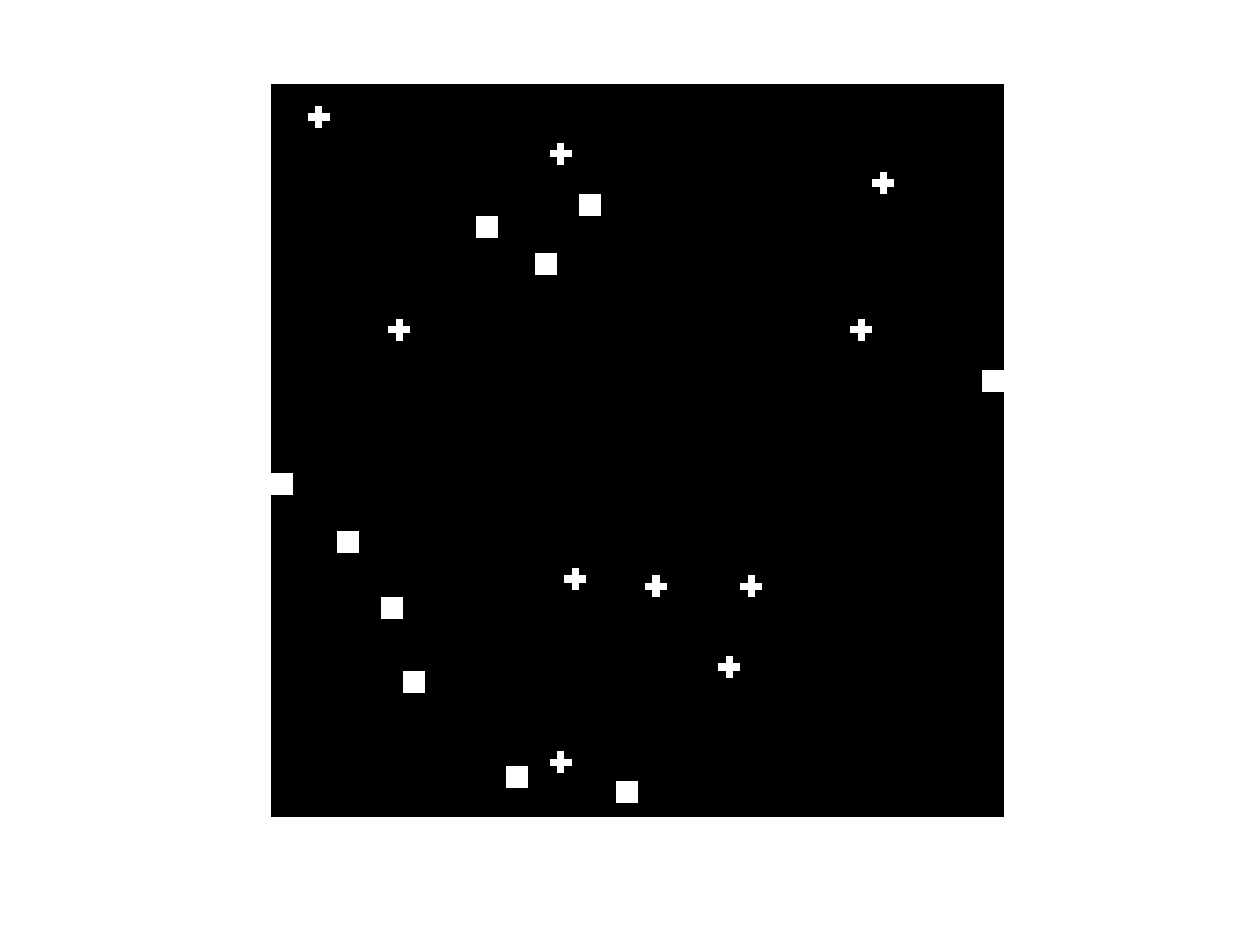
\includegraphics{data/tex/erosionSrc-inc.eps}
\end{picture}
%
\begin{picture}(400,432)(0,0)%(576,432)(0,0)
\end{picture}
}\scalebox{0.45}{% Title: glps_renderer figure
% Creator: GL2PS 1.3.8, (C) 1999-2012 C. Geuzaine
% For: Octave
% CreationDate: Tue Nov 18 11:12:08 2014
\setlength{\unitlength}{1pt}
\begin{picture}(0,0)
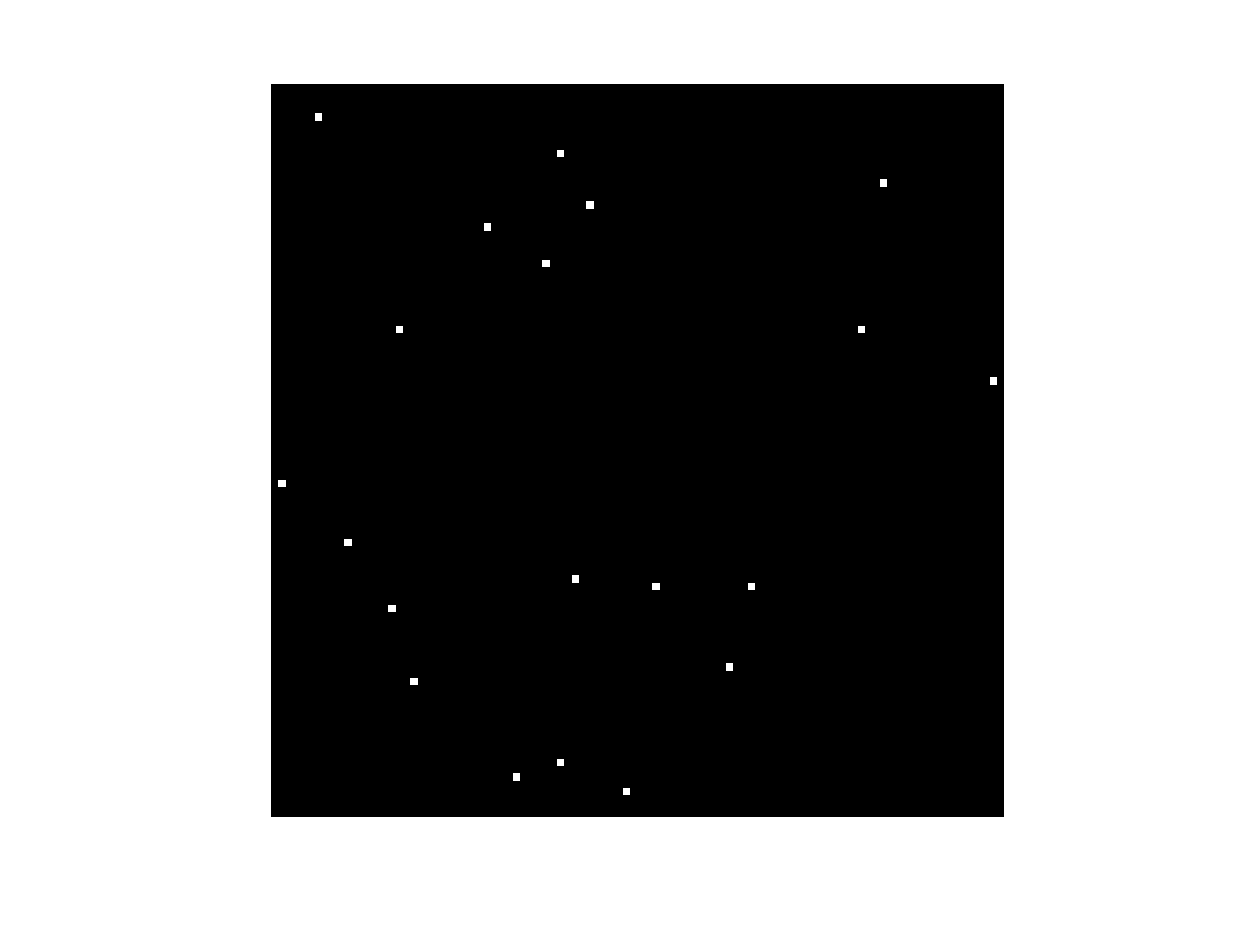
\includegraphics{data/tex/erosion-inc.eps}
\end{picture}%
\begin{picture}(400,432)(0,0)
\end{picture}
}
	\caption{Image d'origine a gauche et resultat de l'erosion par la boule unite au sens du 4-voisinage a droite}
	\label{erosion}
\end{figure}

\begin{figure}[h]
	\centering
	\scalebox{0.45}{% Title: glps_renderer figure
% Creator: GL2PS 1.3.8, (C) 1999-2012 C. Geuzaine
% For: Octave
% CreationDate: Tue Nov 18 11:13:19 2014
\setlength{\unitlength}{1pt}
\begin{picture}(0,0)
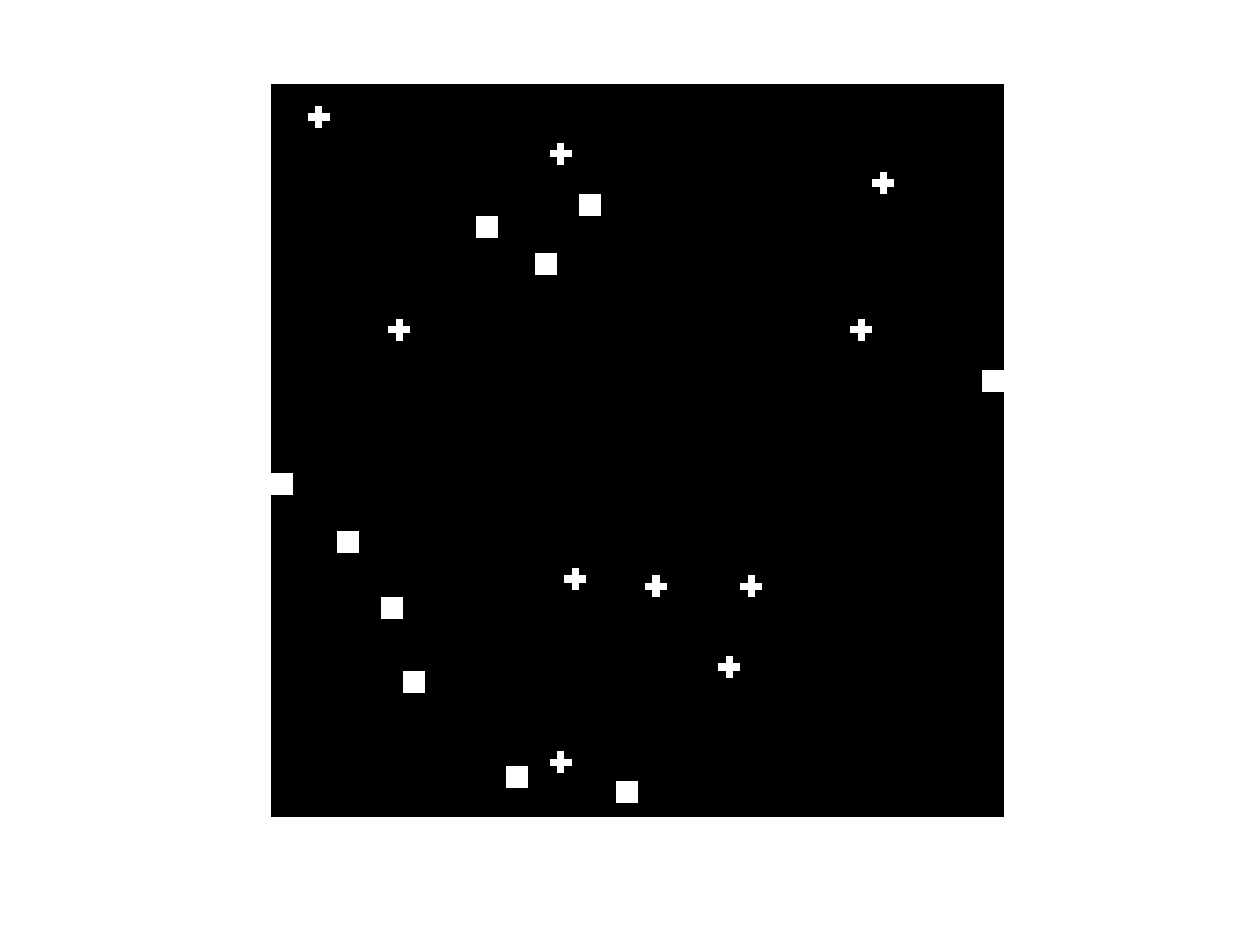
\includegraphics{data/tex/dilatationSrc-inc.eps}
\end{picture}%
\begin{picture}(400,432)(0,0)
\end{picture}
}\scalebox{0.45}{% Title: glps_renderer figure
% Creator: GL2PS 1.3.8, (C) 1999-2012 C. Geuzaine
% For: Octave
% CreationDate: Tue Nov 18 11:13:20 2014
\setlength{\unitlength}{1pt}
\begin{picture}(0,0)
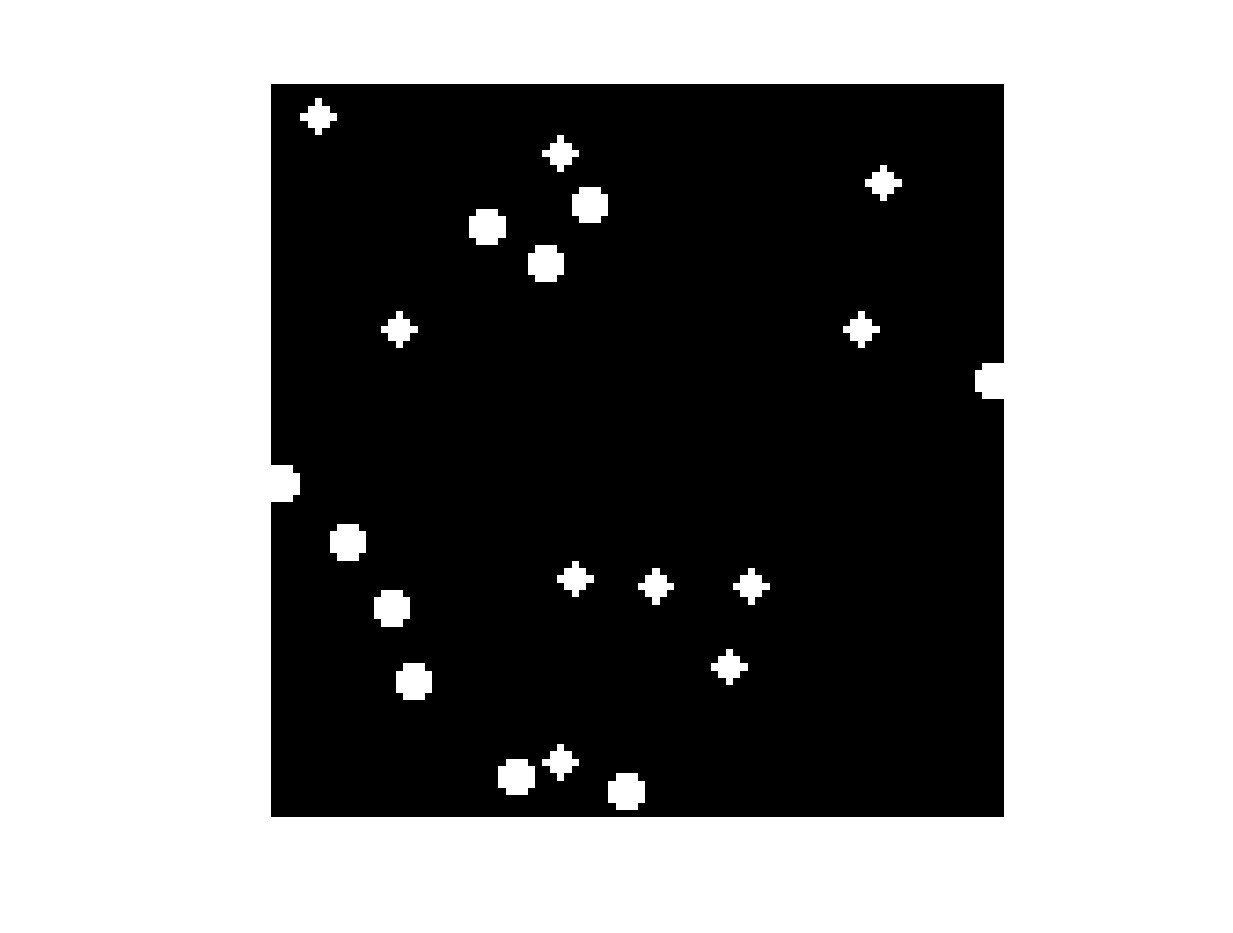
\includegraphics{data/tex/dilatation-inc.eps}
\end{picture}%
\begin{picture}(400,432)(0,0)
\end{picture}
}
	\caption{Image d'origine a gauche et r\'{e}sultat de la dilatation par la boule unit\'{e} au sens du 4-voisinage a droite}
	\label{dilatation}
\end{figure}




\clearpage
\section{Ouverture, fermeture, squel\'{e}tisation}

Les op\'{e}rateurs d'ouverture $\mathcal{O}$, de fermeture $\mathcal{F}$ et de sequ\'{e}letisation $\mathcal{S}$ sont respectivement defini comme suit : 

\begin{align*}	
	X\circ B &=  D_{B^t}\left(E_{B}\left(X\right)\right) \\
	X\bullet B &= E_{B^t}\left(D_{B}\left(X\right)\right) \\
	\mathcal{S}_{B}\left(X\right) &= \underset{n\in \mathbb{N}}{\cup} \left(E_{B_n}\left(X\right) \backslash \left(E_{B_n}\left(X\right)\right)\circ B \right)
\end{align*}
o\`{u} $B_n =\underset{n fois}{\underbrace{B\oplus\ldots\oplus B}}$ et par convention $B_0$ est l'ensemble de un pixel \`{a} l'origine. En pratique, on ne fait pas tendre $n$ vers $+\infty$, mais on s'arr\^{e}te quand on atteint idempotence.

Quelques propri\'{e}t\'{e}s de l'ouverture et de la fermeture
\begin{itemize}
	\item croissance : $X\subset Y \Rightarrow X\bullet B \subset Y\bullet B \text{ et } X\circ B \subset Y\circ B$
	\item idempotence : $\left( X\bullet B \right) \bullet B = X\bullet B $ et $\left( X \circ B \right) \circ B = X\circ B $
	\item dualit\'{e} : $ X\bullet B = \overline{ \overline{X}\circ B}$ et $ X\circ B = \overline{ \overline{X}\bullet B}$
\end{itemize}

Pour d\'{e}montrer ces propri\'{e}t\'{e}s, il suffit de les ecrire avec les definitions... ce qui peut etre un exercice.


\begin{figure}[h]
\hspace{-0.2\textwidth}% Title: glps_renderer figure
% Creator: GL2PS 1.3.8, (C) 1999-2012 C. Geuzaine
% For: Octave
% CreationDate: Fri Nov 21 18:31:21 2014
\setlength{\unitlength}{1pt}
\begin{picture}(0,0)
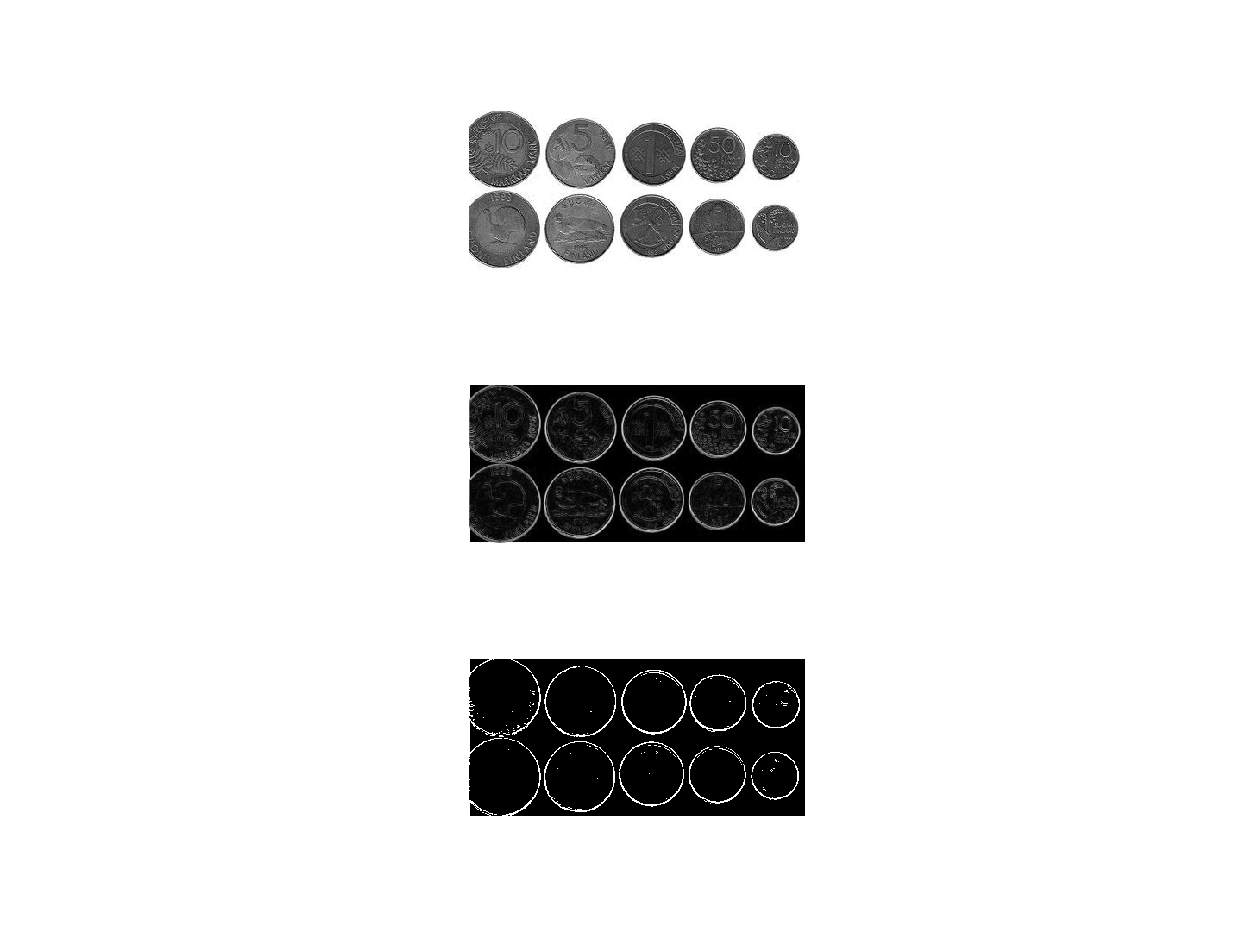
\includegraphics{data/tex/piece-inc}
\end{picture}%
\begin{picture}(576,432)(0,0)
\fontsize{10}{0}
\selectfont\put(298.08,396.743){\makebox(0,0)[b]{\textcolor[rgb]{0,0,0}{{image originale}}}}
\fontsize{10}{0}
\selectfont\put(298.08,265.223){\makebox(0,0)[b]{\textcolor[rgb]{0,0,0}{{Norme du gradient}}}}
\fontsize{10}{0}
\selectfont\put(298.08,133.703){\makebox(0,0)[b]{\textcolor[rgb]{0,0,0}{{Contours}}}}
\end{picture}

	\caption{Image d'origine en haut, image de la norme du gradient au milieu et, en bas, image binaire des contours (seuillage de la norme du gradient \`{a} 100)}
	\label{piece}
\end{figure}

\begin{figure}[h]
\hspace{-0.2\textwidth}% Title: glps_renderer figure
% Creator: GL2PS 1.3.8, (C) 1999-2012 C. Geuzaine
% For: Octave
% CreationDate: Fri Nov 21 18:31:21 2014
\setlength{\unitlength}{1pt}
\begin{picture}(0,0)
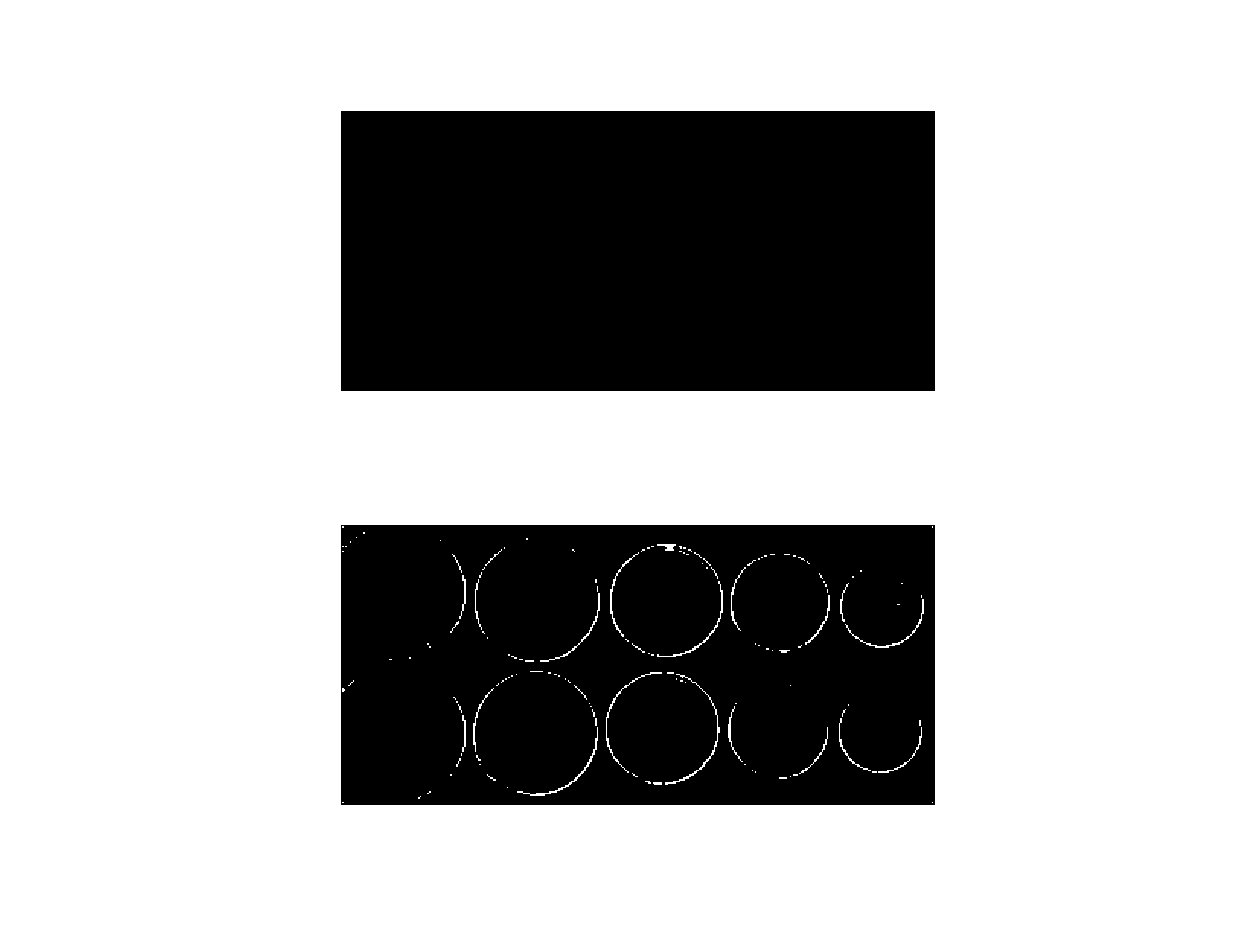
\includegraphics{data/tex/pieceOF-inc}
\end{picture}%
\begin{picture}(576,432)(0,0)
\fontsize{10}{0}
\selectfont\put(298.08,396.743){\makebox(0,0)[b]{\textcolor[rgb]{0,0,0}{{Ouverture}}}}
\fontsize{10}{0}
\selectfont\put(298.08,198.023){\makebox(0,0)[b]{\textcolor[rgb]{0,0,0}{{Fermeture}}}}
\end{picture}

\caption{En haut) image ouverte, en bas) image ferm\'{e}e}
\label{pieceOF}
\end{figure}
%\includegraphics[width=0.45\textwidth]{data/pics/erosionSrc.tex}

\begin{figure}[h]
\hspace{-0.2\textwidth}% Title: glps_renderer figure
% Creator: GL2PS 1.3.8, (C) 1999-2012 C. Geuzaine
% For: Octave
% CreationDate: Tue Nov 18 19:39:51 2014
\setlength{\unitlength}{1pt}
\begin{picture}(0,0)
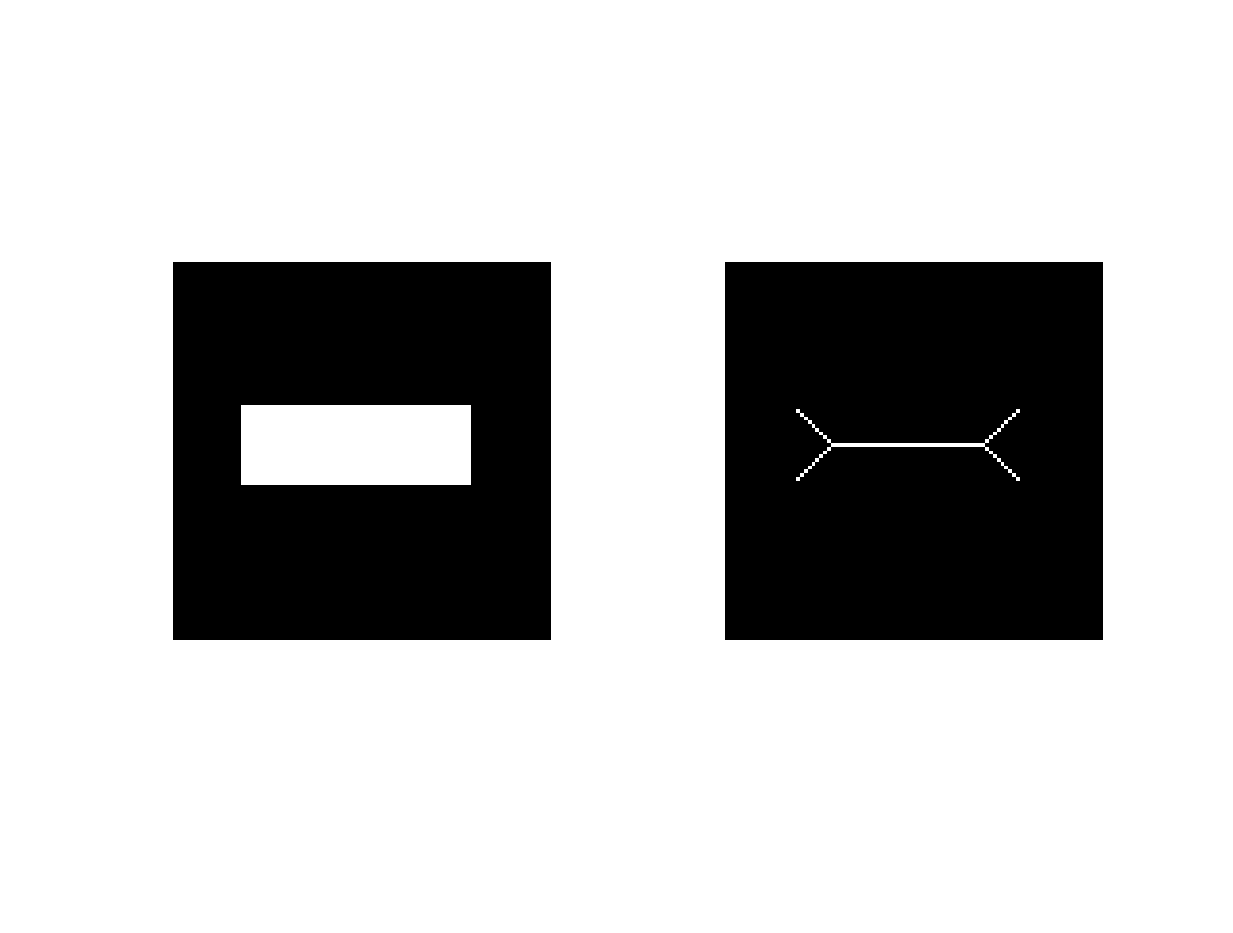
\includegraphics{data/tex/rectSkel-inc}
\end{picture}%
\begin{picture}(450,432)(0,0)
\fontsize{10}{0}
\selectfont\put(165.6,324.28){\makebox(0,0)[b]{\textcolor[rgb]{0,0,0}{{image originale}}}}
\fontsize{10}{0}
\selectfont\put(430.56,324.28){\makebox(0,0)[b]{\textcolor[rgb]{0,0,0}{{squelette}}}}
\end{picture}

\vspace{-40mm}
	\caption{Image d'origine, un rectangle, \`{a} gauche, et, \`{a} droite, le squelette.}
	\label{rectSkel}
\end{figure}
\begin{figure}[h]
\hspace{-0.2\textwidth}% Title: glps_renderer figure
% Creator: GL2PS 1.3.8, (C) 1999-2012 C. Geuzaine
% For: Octave
% CreationDate: Tue Nov 18 19:39:58 2014
\setlength{\unitlength}{1pt}
\begin{picture}(0,0)
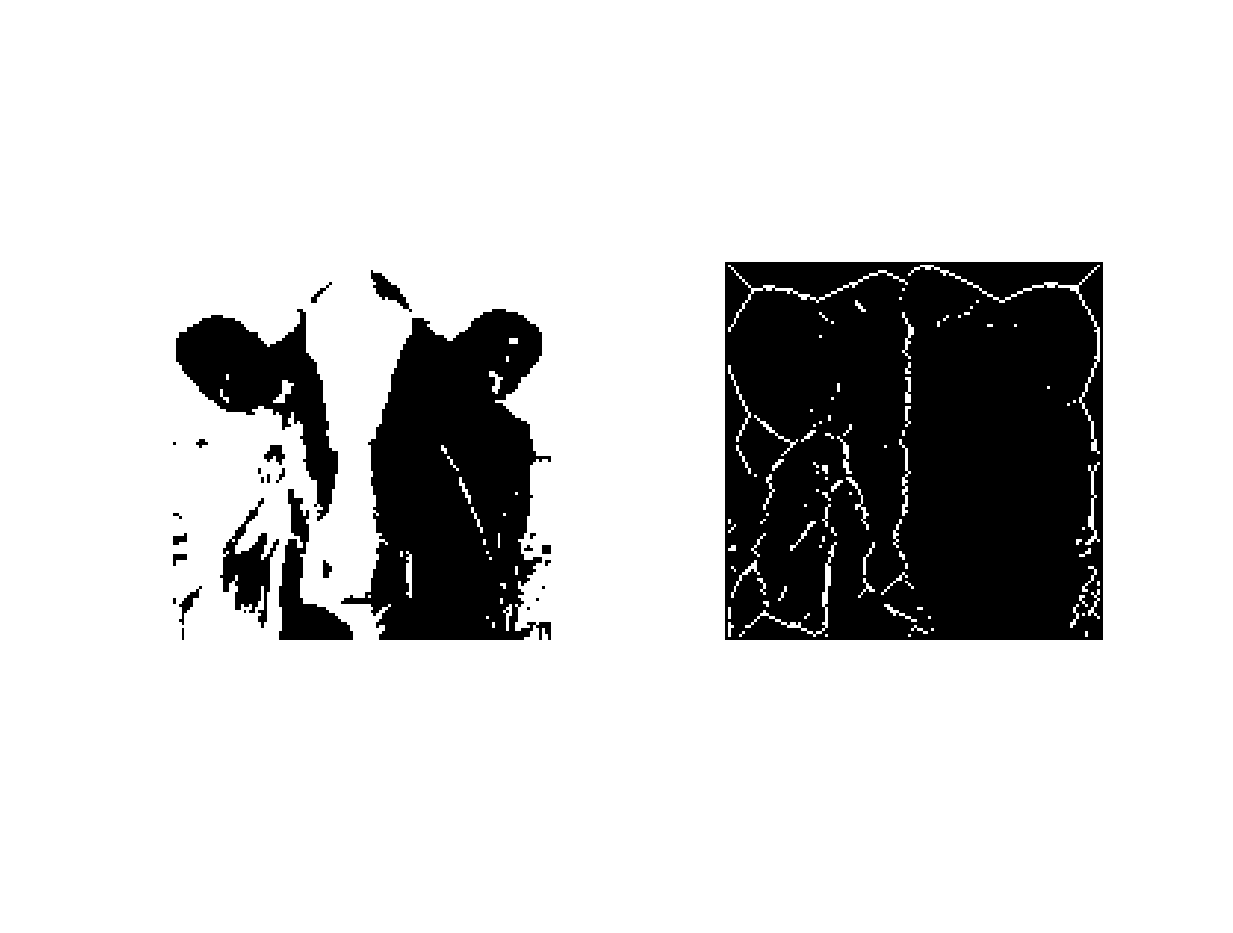
\includegraphics{data/tex/veauSkel-inc}
\end{picture}%
\begin{picture}(450,432)(0,0)
\fontsize{10}{0}
\selectfont\put(165.6,324.28){\makebox(0,0)[b]{\textcolor[rgb]{0,0,0}{{image petit veau}}}}
\fontsize{10}{0}
\selectfont\put(430.56,324.28){\makebox(0,0)[b]{\textcolor[rgb]{0,0,0}{{squelette du petit veau}}}}
\end{picture}

\vspace{-40mm}
	\caption{Image de veau segment\'{e}e, \`{a} gauche, et, \`{a} droite, le squelette.}
	\label{rectSkel}
\end{figure}

\clearpage

\subsection{Hit or Miss Transform}

Ou sous son nom fran\c{}ais, la transform\'{e}e tout-ou-rien. Elle sert \`{a} extraire des motifs d'une image, par exemple les points qui sont \`{a} la fois dans l'objet et qui n'ont aucun voisin (il faut pr\'{e}ciser le voisinage utilis\'{e}). Formellement, on la d\'{e}finit comme suit : 
\begin{displaymath}
	X\odot B = E_{B{\text{fg}}}\left(X\right) \cap E_{B{\text{bg}}}\left(\overline{X}\right)
\end{displaymath}
avec $B = \left(B{\text{fg}},B{\text{bg}}\right)$, ou $B{\text{fg}}$ repr\'{e}sente l'op\'{e}ration sur l'objet et $B{\text{bg}}$ l'op\'{e}ration sur le fond. Les deux \'{e}l\'{e}ments structurants doivent satisfaire $B{\text{fg}}\cap B{\text{bg}} = \varnothing$

\subsubsection{Applications}

\paragraph{Points isol\'{e}s}
Au sens du 4-voisinage, des points isol\'{e}s sont des points qui sont dans l’objet et qui n'ont pas de voisins sur le 4-voisinage, ainsi, on d\'{e}finit les \'{e}l\'{e}ments structurants : 


\begin{displaymath}
B_{\text{fg}} = 
\begin{array}{|c|c|c|}
	\hline 0  & 0  & 0   \\
	\hline 0  & 1  & 0  \\
	\hline 0  & 0  & 0  \\
	\hline
\end{array}
\text{ et } 
B_{\text{bg}} = 
	\begin{array}{|c|c|c|}
	 \hline 0  & 1  & 0   \\
	 \hline 1  & 0  & 1  \\
	 \hline 0  & 1  & 0  \\
	\hline
	\end{array}
\end{displaymath}


on verifie bien que $B{\text{fg}}\cap B{\text{bg}} = \varnothing$. Voici le r\'{e}sultats figure~\ref{points} sur laquelle les points isol\'{e}s figurent en rouge, pour une image de contour binaris\'{e}e (fig.~\ref{piece}).
\begin{figure}[h]
\hspace{0.05\textwidth}\scalebox{0.66}{% Title: glps_renderer figure
% Creator: GL2PS 1.3.8, (C) 1999-2012 C. Geuzaine
% For: Octave
% CreationDate: Tue Nov 18 20:32:12 2014
\setlength{\unitlength}{1pt}
\begin{picture}(0,0)
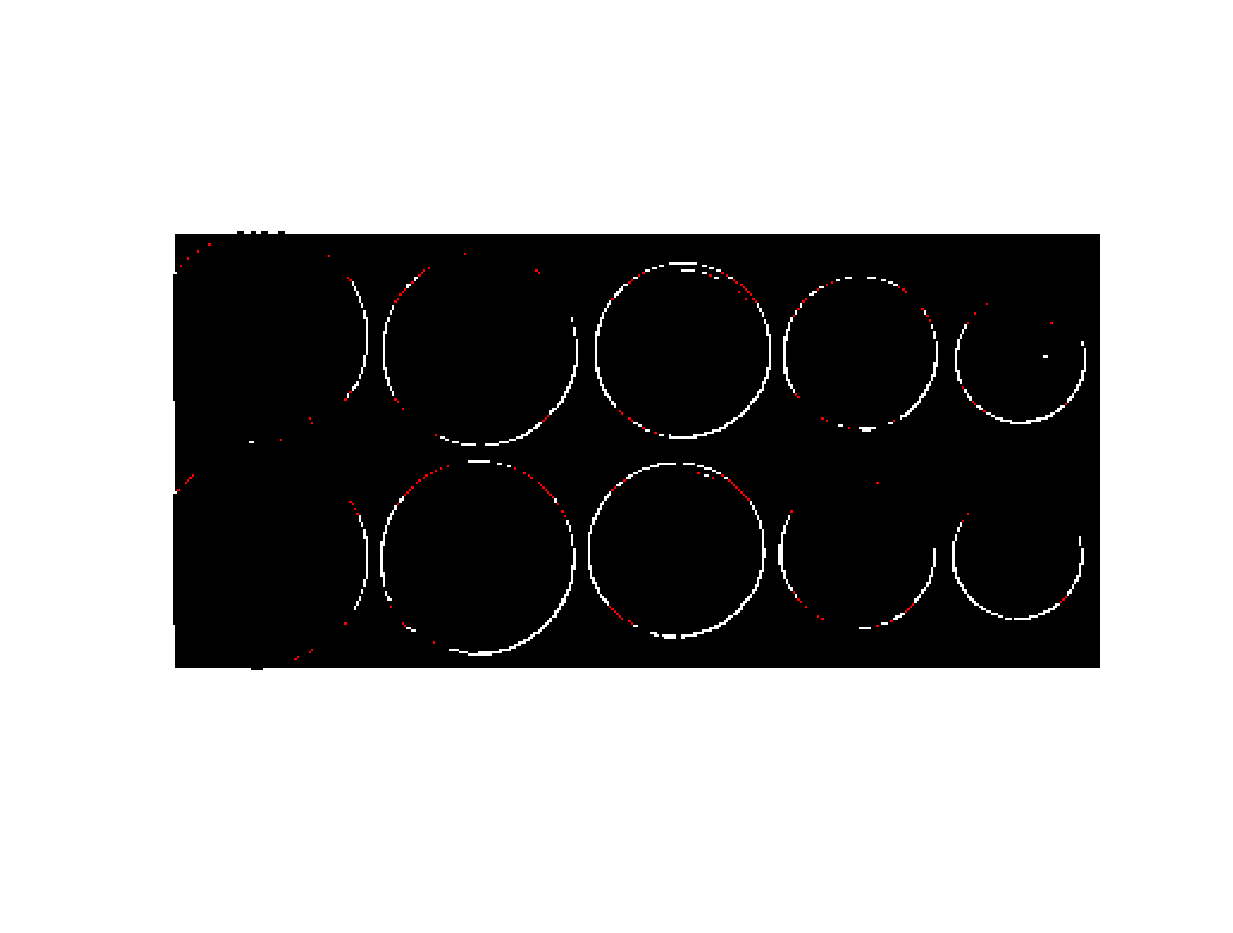
\includegraphics{data/tex/points-inc}
\end{picture}%
\begin{picture}(576,432)(0,0)
\end{picture}
}
\vspace{-25mm}
	\caption{Les points rouge sont isol\'{e}s au sens du 4-voisinage.}
	\label{points}
\end{figure}
\clearpage

\paragraph{Extremit\'{e}s} 
La d\'{e}tection des extr\'{e}mit\'{e}s est plus subtile car il faut consid\'{e}rer plusieurs cas. Ici, on cherche \`{a}{  d\'{e}tecter les extr\'{e}mit\'{e}s au sens du 8-voisinage. Il faut extraire tout les points qui sont dans l'objet et qui n'ont qu'un seul voisin. Pour cela, on va faire plusieurs extractions et le r\'{e}sultat final sera l'union de touts les r\'{e}sultats. Figure~\ref{wodka} montre le r\'{e}sultat de cette op\'{e}ration en rouge sur l'image (les points ont \'{e}t\'{e}s dilat\'{e}s pour plus de claret\'{e}).

Voici les masque utilises : 
\begin{displaymath}
B_{\text{fg}} = 
\begin{array}{|c|c|c|}
	\hline 0  & 0  & 0   \\
	\hline 0  & 1  & 0  \\
	\hline 0  & 0  & 0  \\
	\hline
\end{array}
\end{displaymath}
et
\begin{displaymath}
B_{\text{bg}} \in\left\{ 
	\begin{array}{|c|c|c|}
	 \hline 1  & 0  & 1   \\
	 \hline 1  & 0  & 1  \\
	 \hline 1  & 1  & 1  \\
	\hline
	\end{array},
	\begin{array}{|c|c|c|}
	 \hline 0  & 1  & 1   \\
	 \hline 1  & 0  & 1  \\
	 \hline 1  & 1  & 1  \\
	\hline
	\end{array},
	\begin{array}{|c|c|c|}
	 \hline 1  & 1  & 1   \\
	 \hline 0  & 0  & 1  \\
	 \hline 1  & 1  & 1  \\
	\hline
	\end{array},
	\begin{array}{|c|c|c|}
	 \hline 1  & 1  & 1   \\
	 \hline 1  & 0  & 1  \\
	 \hline 0  & 1  & 1  \\
	\hline
	\end{array},
	\begin{array}{|c|c|c|}
	 \hline 1  & 1  & 1   \\
	 \hline 1  & 0  & 1  \\
	 \hline 1  & 0  & 1  \\
	\hline
	\end{array},
	\begin{array}{|c|c|c|}
	 \hline 1  & 1  & 1   \\
	 \hline 1  & 0  & 1  \\
	 \hline 1  & 1  & 0  \\
	\hline
	\end{array},
	\begin{array}{|c|c|c|}
	 \hline 1  & 1  & 1   \\
	 \hline 1  & 0  & 0  \\
	 \hline 1  & 1  & 1  \\
	\hline
	\end{array},
	\begin{array}{|c|c|c|}
	 \hline 1  & 1  & 0   \\
	 \hline 1  & 0  & 1  \\
	 \hline 1  & 1  & 1  \\
	\hline
	\end{array}
\right\}
\end{displaymath}

\begin{figure}[h]
\hspace{-0.0\textwidth}\scalebox{0.66}{% Title: glps_renderer figure
% Creator: GL2PS 1.3.8, (C) 1999-2012 C. Geuzaine
% For: Octave
% CreationDate: Tue Nov 18 20:52:25 2014
\setlength{\unitlength}{1pt}
\begin{picture}(0,0)
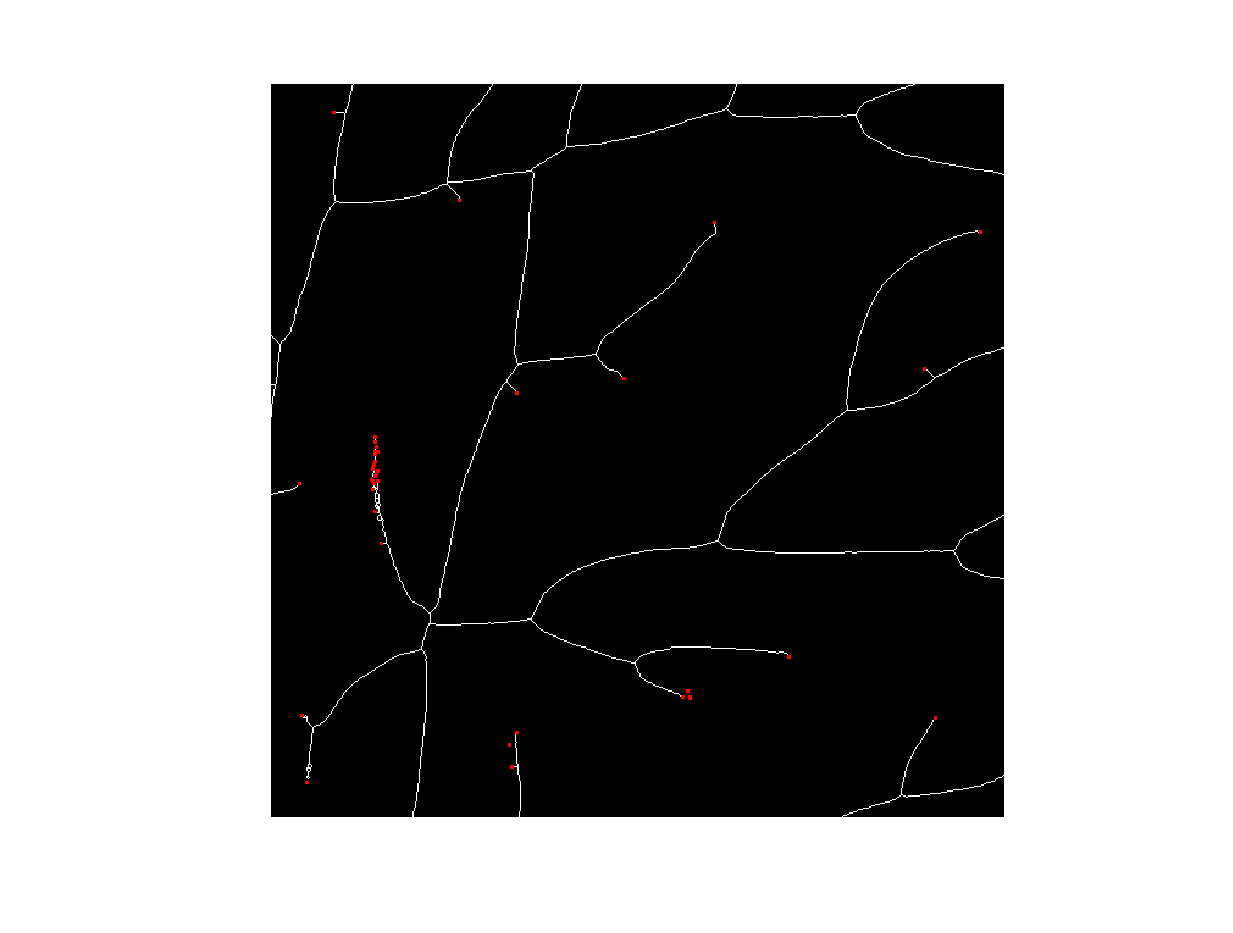
\includegraphics{data/tex/wodka-inc}
\end{picture}%
\begin{picture}(576,432)(0,0)
\end{picture}
}
\vspace{-10mm}
	\caption{Les points rouge sont les extr\'{e}mit\'{e}s au sens du 8-voisinage.}
	\label{wodka}
\end{figure}
\clearpage

\paragraph{D\'{e}tection de contour et comparaison}
On introduit la notion de gradient morphologique $G_B$comme la diff\'{e}rence entre la dilatation et l'\'{e}rosion d'une image par un \'{e}l\'{e}ment structurant B.
\begin{displaymath}
G_B\left(X\right) = D_B\left(X\right)\backslash E_B\left(X\right) \text{ avec, dans notre exemple : }
B = 
\begin{array}{|c|c|c|}
	\hline 0  & 1  & 0   \\
	\hline 1  & 1  & 1  \\
	\hline 0  & 1  & 0  \\
	\hline
\end{array}
\end{displaymath}

En suivant la m\^{e}me logique qu'au paragraphe pr\'{e}c\'{e}dent, on d\'{e}finit aussi les pairs structurantes pour la d\'{e}tection de contours par transformation Tout-ou-Rien : 
\begin{displaymath}
B_{\text{fg}} = 
\begin{array}{|c|c|c|}
	\hline 0  & 0  & 0   \\
	\hline 0  & 1  & 0  \\
	\hline 0  & 0  & 0  \\
	\hline
\end{array}
\end{displaymath}
et
\begin{displaymath}
B_{\text{bg}} \in\left\{ 
	\begin{array}{|c|c|c|}
	 \hline 0  & 1  & 0   \\
	 \hline 0  & 0  & 0  \\
	 \hline 0  & 0  & 0  \\
	\hline
	\end{array},
	\begin{array}{|c|c|c|}
	 \hline 0  & 0  & 0   \\
	 \hline 1  & 0  & 0  \\
	 \hline 0  & 0  & 0  \\
	\hline
	\end{array},
	\begin{array}{|c|c|c|}
	 \hline 0  & 0  & 0   \\
	 \hline 0  & 0  & 0  \\
	 \hline 0  & 1  & 0  \\
	\hline
	\end{array},
	\begin{array}{|c|c|c|}
	 \hline 0  & 0  & 0   \\
	 \hline 0  & 0  & 1  \\
	 \hline 0  & 0  & 0  \\
	\hline
	\end{array}
\right\}
\end{displaymath}

Figure~\ref{gradient} et figure~\ref{contour} repr\'{e}sentent les r\'{e}sultats respectifs du gradient morphologique et de la d\'{e}tection par transform\'{e}e Tout-ou-Rien en pixel rouge.

\begin{figure}[h]
\hspace{-0.0\textwidth}\scalebox{0.66}{% Title: glps_renderer figure
% Creator: GL2PS 1.3.8, (C) 1999-2012 C. Geuzaine
% For: Octave
% CreationDate: Tue Nov 18 21:28:43 2014
\setlength{\unitlength}{1pt}
\begin{picture}(0,0)
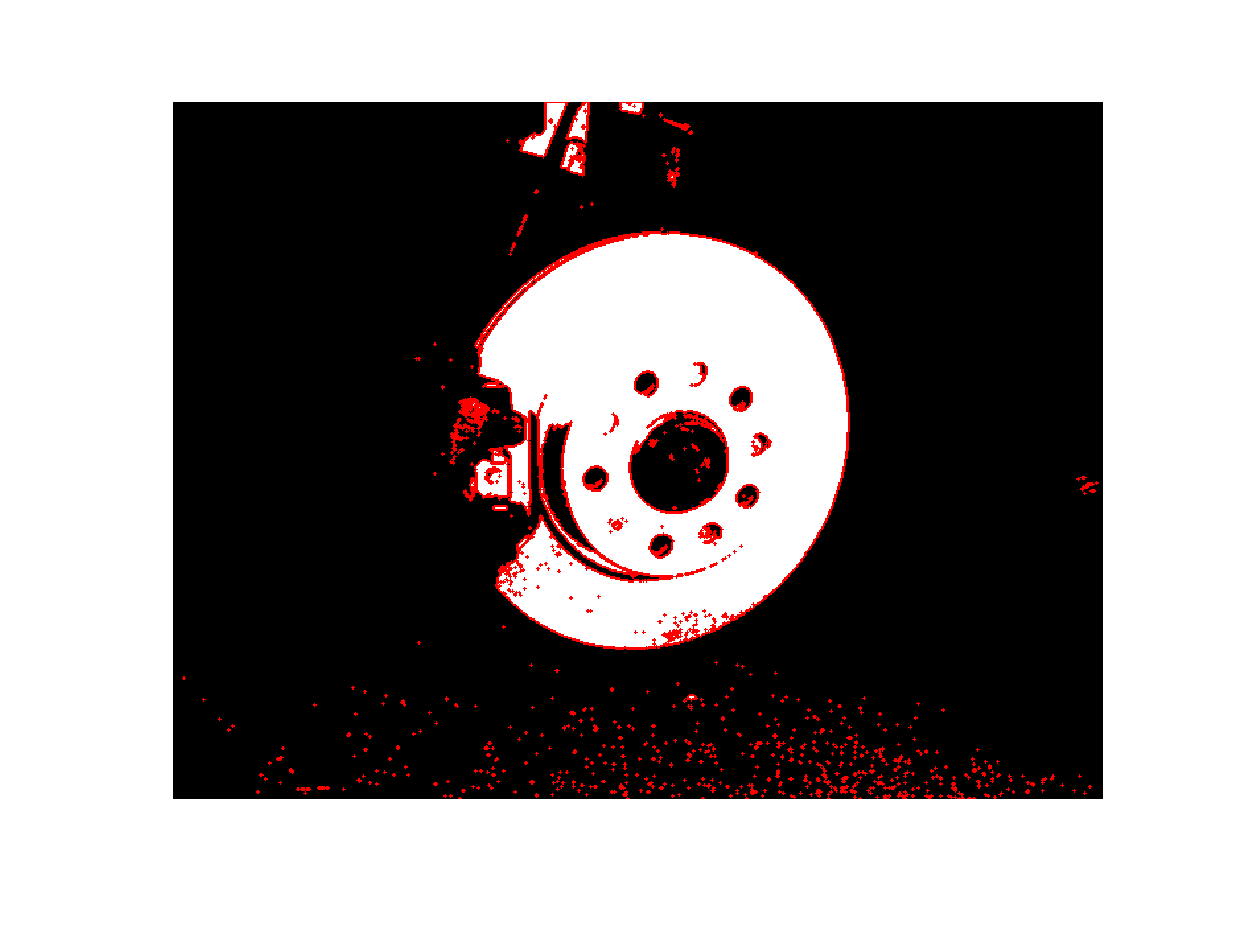
\includegraphics{data/tex/gradient-inc}
\end{picture}%
\begin{picture}(576,432)(0,0)
\fontsize{10}{0}
\selectfont\put(298.08,400.96){\makebox(0,0)[b]{\textcolor[rgb]{0,0,0}{{gradient morphologique}}}}
\end{picture}
}
\vspace{-10mm}
	\caption{Les points rouges sont les contours au sens du gradient morphologique}
	\label{gradient}
\end{figure}

\begin{figure}[h]
\hspace{-0.0\textwidth}\scalebox{0.66}{% Title: glps_renderer figure
% Creator: GL2PS 1.3.8, (C) 1999-2012 C. Geuzaine
% For: Octave
% CreationDate: Tue Nov 18 21:28:44 2014
\setlength{\unitlength}{1pt}
\begin{picture}(0,0)
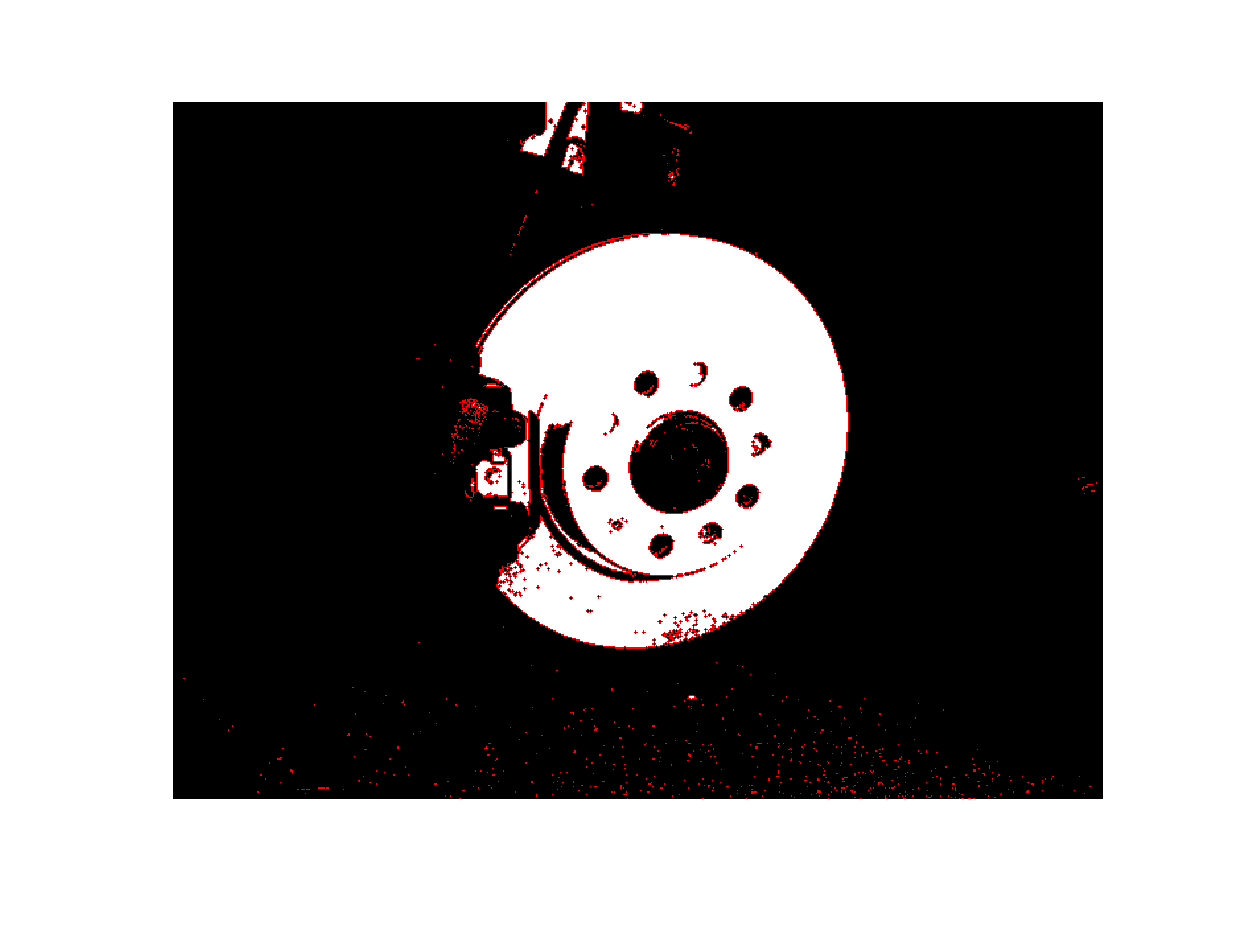
\includegraphics{data/tex/contour-inc}
\end{picture}%
\begin{picture}(576,432)(0,0)
\fontsize{10}{0}
\selectfont\put(298.08,400.96){\makebox(0,0)[b]{\textcolor[rgb]{0,0,0}{{Hit or Miss method}}}}
\end{picture}
}
\vspace{-10mm}
	\caption{Les points rouges sont les contours au sens de la transformee Tout-ou-Rien}
	\label{contour}
\end{figure}

\clearpage

\subsection{Lien entre dilatation et carte de distance}
La dilatation d'une image a d\'{e}j\`{a} \'{e}t\'{e} introduite, il ne reste que la notion de carte de distance. C'est tout simplement une image qui en chaque point donne la distance \~{a} l'objet le plus proche. Elle est impl\'{e}ment\'{e}e dans l'op\'{e}rateur \textit{bwdist} sous \textit{octave}

La figure~\ref{distanceAndDilatation} montre le r\'{e}sultat d'une dilatation par la m\'{e}thode utilisant la somme de Minkowski (la ligne du haut) et le seuillage de la carte de distance.

\begin{figure}[h]
\hspace{-0.0\textwidth}\scalebox{0.66}{% Title: glps_renderer figure
% Creator: GL2PS 1.3.8, (C) 1999-2012 C. Geuzaine
% For: Octave
% CreationDate: Tue Nov 18 11:19:22 2014
\setlength{\unitlength}{1pt}
\begin{picture}(0,0)
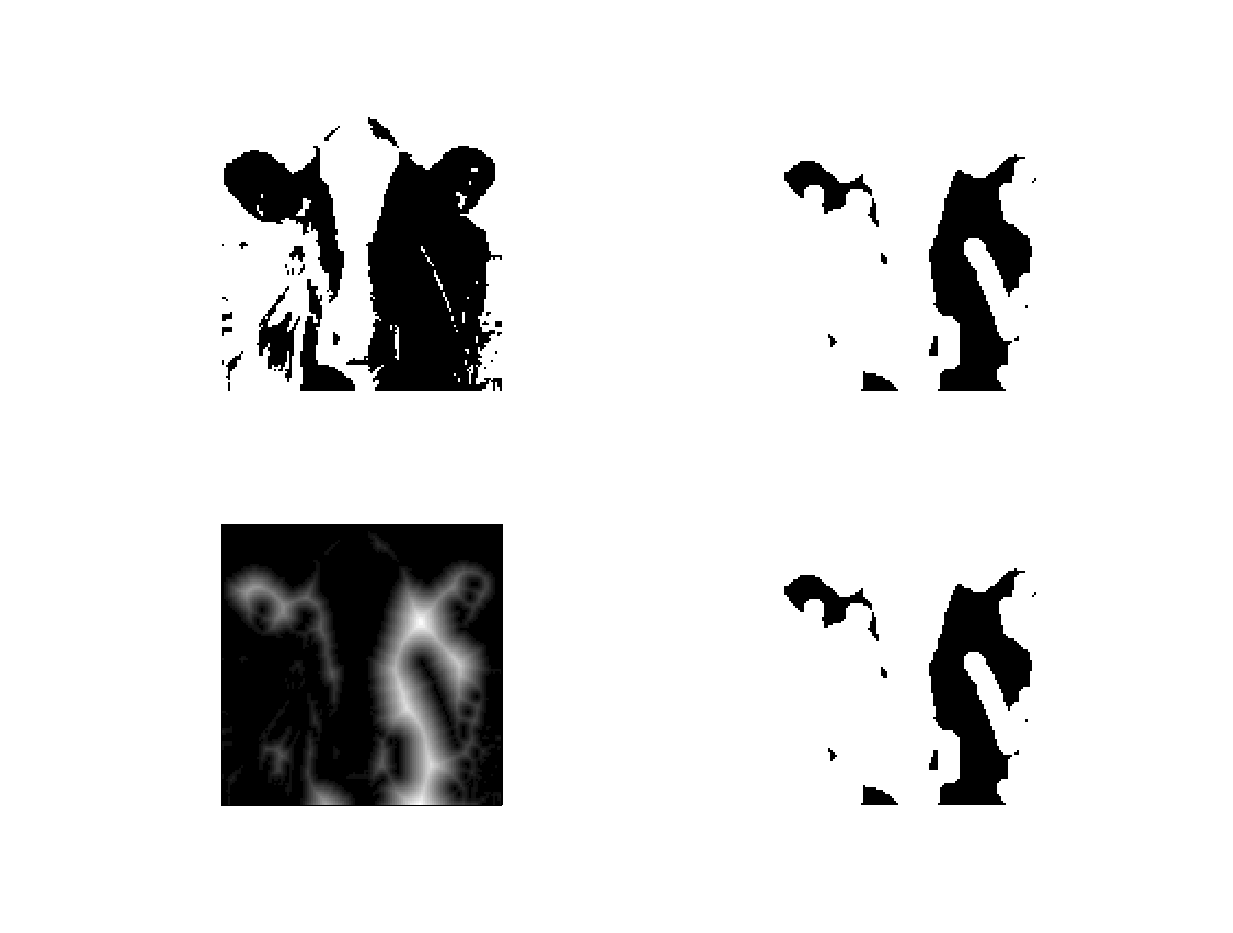
\includegraphics{data/tex/distanceAndDilatation-inc.eps}
\end{picture}%
\begin{picture}(576,432)(0,0)
\fontsize{10}{0}
\selectfont\put(165.6,396.743){\makebox(0,0)[b]{\textcolor[rgb]{0,0,0}{{Image originale}}}}
\fontsize{10}{0}
\selectfont\put(430.56,396.743){\makebox(0,0)[b]{\textcolor[rgb]{0,0,0}{{Image dilatee par une boule de rayon 5}}}}
\fontsize{10}{0}
\selectfont\put(118.831,48.5153){\makebox(0,0)[t]{\textcolor[rgb]{0,0,0}{{20}}}}
\fontsize{10}{0}
\selectfont\put(139.851,48.5153){\makebox(0,0)[t]{\textcolor[rgb]{0,0,0}{{40}}}}
\fontsize{10}{0}
\selectfont\put(160.871,48.5153){\makebox(0,0)[t]{\textcolor[rgb]{0,0,0}{{60}}}}
\fontsize{10}{0}
\selectfont\put(181.89,48.5153){\makebox(0,0)[t]{\textcolor[rgb]{0,0,0}{{80}}}}
\fontsize{10}{0}
\selectfont\put(202.91,48.5153){\makebox(0,0)[t]{\textcolor[rgb]{0,0,0}{{100}}}}
\fontsize{10}{0}
\selectfont\put(223.929,48.5153){\makebox(0,0)[t]{\textcolor[rgb]{0,0,0}{{120}}}}
\fontsize{10}{0}
\selectfont\put(93.355,167.529){\makebox(0,0)[r]{\textcolor[rgb]{0,0,0}{{20}}}}
\fontsize{10}{0}
\selectfont\put(93.355,146.509){\makebox(0,0)[r]{\textcolor[rgb]{0,0,0}{{40}}}}
\fontsize{10}{0}
\selectfont\put(93.355,125.49){\makebox(0,0)[r]{\textcolor[rgb]{0,0,0}{{60}}}}
\fontsize{10}{0}
\selectfont\put(93.355,104.47){\makebox(0,0)[r]{\textcolor[rgb]{0,0,0}{{80}}}}
\fontsize{10}{0}
\selectfont\put(93.355,83.4505){\makebox(0,0)[r]{\textcolor[rgb]{0,0,0}{{100}}}}
\fontsize{10}{0}
\selectfont\put(93.355,62.431){\makebox(0,0)[r]{\textcolor[rgb]{0,0,0}{{120}}}}
\fontsize{10}{0}
\selectfont\put(165.6,198.023){\makebox(0,0)[b]{\textcolor[rgb]{0,0,0}{{carte de distance}}}}
\fontsize{10}{0}
\selectfont\put(430.56,198.023){\makebox(0,0)[b]{\textcolor[rgb]{0,0,0}{{Seuillage de la carte de distance... dilatation}}}}
\end{picture}
}
\vspace{-10mm}
	\caption{}
	\label{distanceAndDilatation}
\end{figure}

\end{document}





